\documentclass{article}

\usepackage[portuguese]{babel}


\usepackage[letterpaper,top=2cm,bottom=2cm,left=3cm,right=3cm,marginparwidth=1.75cm]{geometry}

% Useful packages
\usepackage{amsmath}
\usepackage{multicol}
\usepackage{graphicx}
\usepackage[colorlinks=true, allcolors=blue]{hyperref}
\newtheorem{theorem}{Teorema}[section]
\newtheorem{proof}{Demonstração}[theorem]
\newtheorem{lemma}[theorem]{Lema}

\title{Triângulos}
\author{Télico Oliveira}

\begin{document}
\maketitle
\section{Elementos de um triângulo}
Os três elementos de um triângulo os seus \textbf{}{três vértices}, os seus \textbf{três lados} e os seus \textbf{ângulos}. 
\section{Classificação dos triângulos}
Os triângulos podem ser classificados quanto às medidas dos seus lados ou quanto à medida de abertura dos seus ângulos. 
\subsection{Classificação quanto aos seus ângulos}
Quanto aos seus ângulos, os triângulos podem ser classificados como acutângulos, retângulos ou obtusângulos.  
\\
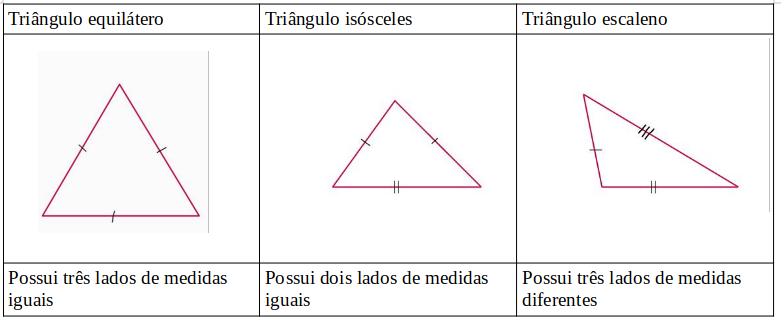
\includegraphics[scale = 0.5]{tabela1.png}


\subsection{Classificação quanto à medida dos seus lados}
Um triângulo pode ainda ser classificado como equilátero, isósceles ou escaleno. 
\\
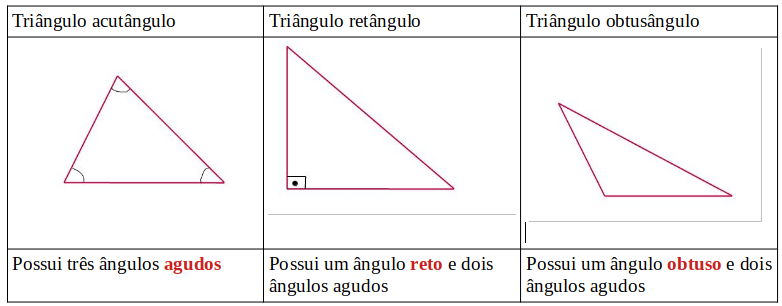
\includegraphics[scale = 0.5]{tabela2.png}
\section{Relação do ângulo externo com os ângulos internos não adjacentes a ele}
\begin{theorem}
A medida de cada ângulo externo  de um triângulo é igual à soma das medidas dos dois ângulos internos não adjacentes a ele. 
\end{theorem}
\subsection{Exercícios resolvidos}
\begin{enumerate}
    \item Calcule o valor de x e y em graus. 
\begin{multicols}{2}

\begin{enumerate}
\item 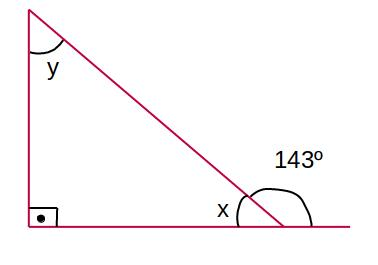
\includegraphics[scale = 0.6]{triangulos1.jpg}
\item 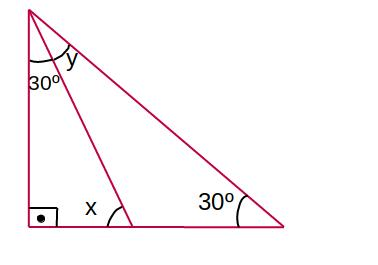
\includegraphics[scale = 0.6]{triangulos2.jpg}
\end{enumerate}
\end{multicols}    
\end{enumerate}

\end{document}